\documentclass[12pt]{article}

\usepackage[utf8]{inputenc}
\usepackage{latexsym,amsfonts,amssymb,amsthm,amsmath, graphicx, float, hyperref}

\setlength{\parindent}{0in}
\setlength{\oddsidemargin}{0in}
\setlength{\textwidth}{6.5in}
\setlength{\textheight}{8.8in}
\setlength{\topmargin}{-0.5in}
\setlength{\headheight}{18pt}



\title{Assignment 1 — Applied Algorithms, T. II/2024–25}
\author{Austin Jetrin Maddison 6481268}

\begin{document}
	
	\maketitle
	
	\vspace{0.5in}
	
	\subsection*{Problem 1. Las Vegas and Monte Carlo}
	
	
	a.i) We want to show the probablity of running time of Monte Carlo is atleast the worst running time which is $4f(n)$. We can use markov inqualities to bound it..
	\\

	\begin{align*}
		\textbf{P}(X \le \lambda ) & \le \frac{ E [ X ] }{ \lambda }\\
	\end{align*}

	\begin{align*}
		\textbf{P}(T(n) \le 4f(n) ) & \le \frac{f(n)}{4f(n)}\\
								    & \le \frac{1}{4}		
	\end{align*}
	
	a.ii) The worse-case running time happens at most 1/4 which produces incorrect answers. We can get the complement of the last answer...    

	\begin{align*}
		1 - \textbf{P}(T(n) \le 4f(n) ) &  \le 1 - \frac{1}{4} = \frac{3}{4}
	\end{align*}
	
	b.i) The LV algorithm running time is described as the follwing. Each iteration requires running A to produce an answer then run C to check the answer. So the running time for each trial is...
	
	\begin{align*}
		\text{1 iteration running time of LV} = f(n) + g(n)
	\end{align*}

	So the question is what is the expected iterations needed to run LV to get a correct answer. If p is the probablity of success then the expected $1/p$.

	\begin{align*}
		\text{Running time of LV} = \frac{1}{p}(f(n) + g(n))
	\end{align*}

	\vspace{2in} %Leave space for comments!
	
	
	\subsection*{Problem 2. Chernoff-Hoeffding With Bounds}
	2.1)
	\begin{align*}
		\mathrm{Pr}[X &> (1+\beta)\mu]\leq\exp\left(-\frac{\beta^{2}}{2+\beta}\mu H\right) \\
		\mathrm{Pr}[X &> (1+\varepsilon)\mu H]\leq\exp\left(-\frac{\varepsilon^{2}}{2+\varepsilon}\mu H\right)
	\end{align*}

	\begin{align*}
		(1 + \epsilon) \mu_{H} &= (1 + \beta) \mu \\
		\frac{\mu_{H}}{\mu} &= \frac{1 + \epsilon}{1 + \beta}\\
		% \beta $= \frac{\mu_{H}(1 + \epsilon)}{\mu}\\
	\end{align*}


	2.2)
	\begin{align*}
		\mathrm{Pr}[X &> (1+\beta)\mu]\leq\exp\left(-\frac{\beta^{2}}{2+\beta}\mu H\right) \\
		\mathrm{Pr}[X &> (1+\varepsilon)\mu H]\leq\exp\left(-\frac{\varepsilon^{2}}{2+\varepsilon}\mu H\right)
	\end{align*}

	\begin{align*}
		(1 + \epsilon) \mu_{H} &= (1 + \beta) \mu \\
		\frac{\mu_{H}}{\mu} &= \frac{1 + \epsilon}{1 + \beta}\\
		% \beta $= \frac{\mu_{H}(1 + \epsilon)}{\mu}\\
	\end{align*}

	2.3)
	\begin{align*}
		\mathrm{Pr}[X &> (1+\beta)\mu]\leq\exp\left(-\frac{\beta^{2}}{2+\beta}\mu H\right) \\
		\mathrm{Pr}[X &> (1+\varepsilon)\mu H]\leq\exp\left(-\frac{\varepsilon^{2}}{2+\varepsilon}\mu H\right)
	\end{align*}

	\begin{align*}
		(1 + \epsilon) \mu_{H} &= (1 + \beta) \mu \\
		\frac{\mu_{H}}{\mu} &= \frac{1 + \epsilon}{1 + \beta}\\
		% \beta $= \frac{\mu_{H}(1 + \epsilon)}{\mu}\\
	\end{align*}
	
	2.4)
	\begin{align*}
		\mathrm{Pr}[X &> (1+\beta)\mu]\leq\exp\left(-\frac{\beta^{2}}{2+\beta}\mu H\right) \\
		\mathrm{Pr}[X &> (1+\varepsilon)\mu H]\leq\exp\left(-\frac{\varepsilon^{2}}{2+\varepsilon}\mu H\right)
	\end{align*}

	\begin{align*}
		(1 + \epsilon) \mu_{H} &= (1 + \beta) \mu \\
		\frac{\mu_{H}}{\mu} &= \frac{1 + \epsilon}{1 + \beta}\\
		% \beta $= \frac{\mu_{H}(1 + \epsilon)}{\mu}\\
	\end{align*}
	\vspace{2in} %Leave space for comments!
	
	
	\subsection*{Problem 3. Rescaling Trick}
	(Statement of problem goes here.)\\
	
	\begin{proof}
		(Type your proof here.)
	\end{proof}
	
	\vspace{2in} %Leave space for comments!
	
	
	
	\subsection*{Problem 4. $x^2$ With $\pi$ Degrees of Freedom}
	(Statement of problem goes here.)\\
	
	\begin{proof}
		(Type your proof here.)
	\end{proof}
	
	\vspace{2in} %Leave space for comments!
	
	
	\subsection*{Problem 5. Simple Samplers.}
	(Statement of problem goes here.)\\
	
	\begin{proof}
		(Type your proof here.)
	\end{proof}
	
	\vspace{2in} %Leave space for comments!
	
	
	\subsection*{Problem 6. Median of Means}
	(Statement of problem goes here.)\\
	
	\begin{proof}
		(Type your proof here.)
	\end{proof}
	
	\vspace{2in} %Leave space for comments!
	
	
	\subsection*{Problem 7. Skip List}
	\vspace{20pt}
	\subsubsection*{Experimental Setup}
	Conducted our benchmarks using Google Benchmark on a system with the following hardware specifications:

\begin{itemize}
    \item \textbf{Processor}: 11th Gen Intel(R) Core(TM) i7-11370H 8-core CPU @ 3.3 GHz
    \item \textbf{Cache Hierarchy}:
    \begin{itemize}
        \item L1 Data: 48 KiB per core (\(\times 4\))
        \item L1 Instruction: 32 KiB per core (\(\times 4\))
        \item L2 Unified: 1280 KiB per core (\(\times 4\))
        \item L3 Unified: 12,288 KiB (shared)
    \end{itemize}
\end{itemize}

All benchmarks were compiled using \texttt{-Ox} optimization level with \texttt{MSVC} (version 19.42.34436) and executed in a single-threaded environment to minimize external interference. Memory usage was measured using the Windows API \texttt{GetProcessMemory()}.\\

\subsubsection*{Questions And Experiments}
	
Q1.) Can we perform count coin tosses differently and is the alternative better?

\begin{figure}[H]
	\centering
	\begin{minipage}{0.32\textwidth}
		\centering
		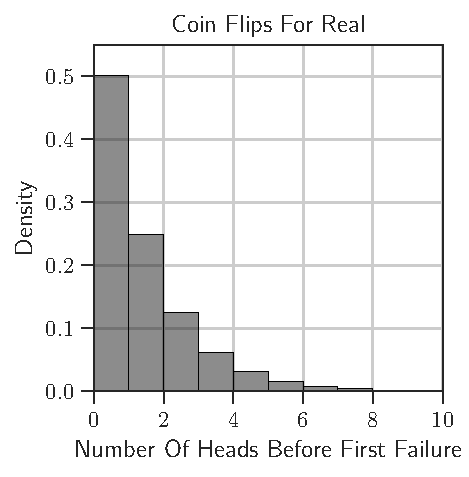
\includegraphics[width=\linewidth]{../notebook/coin_flips_for_real.pdf}
		\label{fig:coin_flips_for_real}
	\end{minipage}\hfill
	\begin{minipage}{0.32\textwidth}
		\centering
		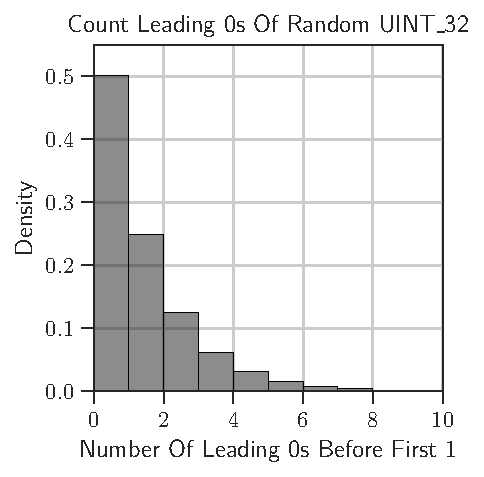
\includegraphics[width=\linewidth]{../notebook/count_leading_0s_of_random_uint_32.pdf}
		\label{fig:coin_flips_count_leading}
	\end{minipage}\hfill
	\begin{minipage}{0.32\textwidth}
		\centering
		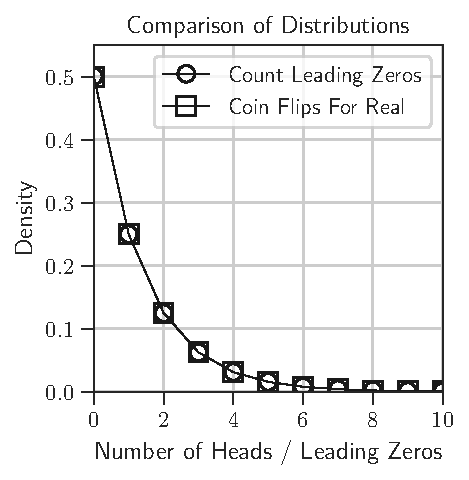
\includegraphics[width=\linewidth]{../notebook/comparison_of_distributions.pdf}
		\label{fig:coin_flips_comparison}
	\end{minipage}
\end{figure}


\begin{table}[h]
	\centering
	\small
	\begin{tabular}{lrrr}
		\hline
		\textbf{Benchmark} & \textbf{Time (ns)} & \textbf{CPU (ns)} & \textbf{Iterations} \\
		\hline
		Coin Flip For Real & 29.8 & 29.3 & 22,400,000 \\
		\hline
		Coin Flip Count Leading 0s & 5.11 & 4.87 & 144,516,129 \\
	\end{tabular}
	\caption{Benchmark results comparing different coin flip implementations.}
	\label{tab:benchmark_results}
\end{table}

Q2.) How does varying max height change performance?

Q3.) Linked lists are known to be cache unfriendly, is there a way we can modify 

Q4.) How does it perform against a reputable ordered map?
\\\\
	
b.) Search algorithm of Skip List when start is at the bottom left corner in $O(\log(d))$ where d is the number of elements smaller than the key?
	

	
	\vspace{2in} %Leave space for comments!
	
	
	
	\subsection*{Problem 8. ($a,b$) tree. ($2, 3$) tree.}

	a.)	
	\begin{figure}[H] 
		\centering
		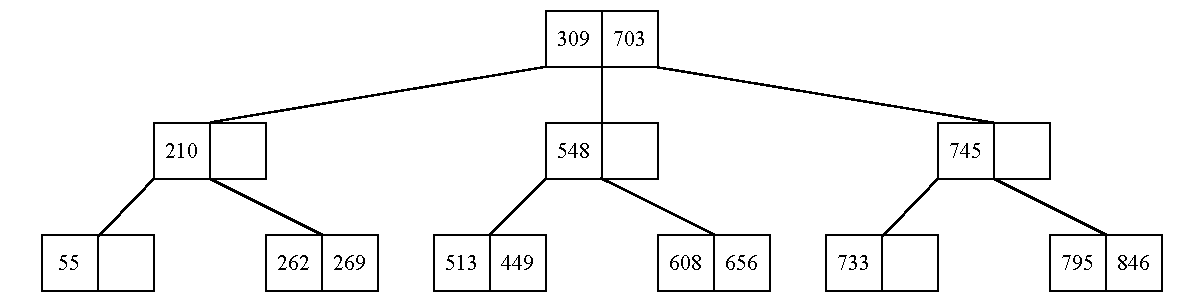
\includegraphics[width=0.9\linewidth]{Q8_a.drawio}
		\caption{Keys $733, 703, 608, 846, 309, 269, 55, 745, 548, 449, 513, 210, 795, 656, 262$ inserted into a $(2, 3)$ tree.}
		\label{fig:q8a}
	\end{figure}
	

	
	b.) 
	\begin{figure}[H] 
		\centering
		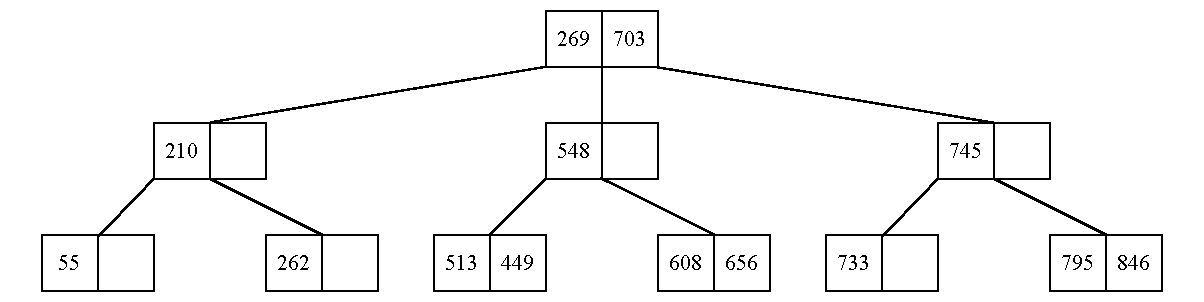
\includegraphics[width=0.9\linewidth]{Q8_b.drawio}
		\caption{Key 309 removed from Figure~\ref{fig:q8a} tree.}
		\label{fig:q8b}
	\end{figure}
	
	
\vspace{2in} %Leave space for comments!


\subsection*{Problem 9. B-Tree Speed}

\subsubsection*{Experimental Setup}
Conducted our benchmarks using Google Benchmark on a system with the following hardware specifications:

\begin{itemize}
	\item \textbf{Processor}: 11th Gen Intel(R) Core(TM) i7-11370H 8-core CPU @ 3.3 GHz
	\item \textbf{Cache Hierarchy}:
	\begin{itemize}
		\item L1 Data: 48 KiB per core (\(\times 4\))
		\item L1 Instruction: 32 KiB per core (\(\times 4\))
		\item L2 Unified: 1280 KiB per core (\(\times 4\))
		\item L3 Unified: 12,288 KiB (shared)
	\end{itemize}
\end{itemize}

All benchmarks were compiled using \texttt{-Ox} optimization level with \texttt{MSVC} (version 19.42.34436) and executed in a single-threaded environment to minimize external interference. Memory usage was measured using the Windows API \texttt{GetProcessMemory()}.\\
\\
The B-Tree implementation utilized in this experiment is sourced from the repository by frozenca
on GitHub~\cite{btree_github}.

\subsubsection*{Finding Optimal Parameter b Of B-Tree}
First I carried out benchmarks to measure performance of tens of millions of random unique keys being inserted into the B-Tree while varying b parameter. 
\begin{table}[h]
	\centering
	\small
	\begin{tabular}{lrrr}
		\hline
		\textbf{b} & \textbf{CPU Time (ms)} & \textbf{Virtual Memory Usage (KB)} & \textbf{Physical Memory Usage (KB)} \\
		\hline
		2    & 59359.375  & 1294456  & 2544788 \\
		4    & 86968.750  & 539168   & 1063908 \\
		6    & 106484.375 & 375208   & 740108  \\
		8    & 123265.625 & 302968   & 596900  \\
		16   & 135156.250 & 202252   & 400248  \\
		32   & 144640.625 & 156320   & 309792  \\
		64   & 153750.000 & 135372   & 268680  \\
		128  & 163312.500 & 129468   & 256996  \\
		256  & 174062.500 & 135368   & 267676  \\
		512  & 186078.125 & 142356   & 280852  \\
		1024 & 200796.875 & 145848   & 285412  \\
		2048 & 221015.625 & 122476   & 246636  \\
		\hline
	\end{tabular}
	\caption{Benchmark results for B-Tree insertion with $20 \times 10^6$ inserts and varying $b$ from 2 to 2048.}
\end{table}

\begin{figure}[H]
	\centering
	\begin{minipage}{1\textwidth}
		\centering
		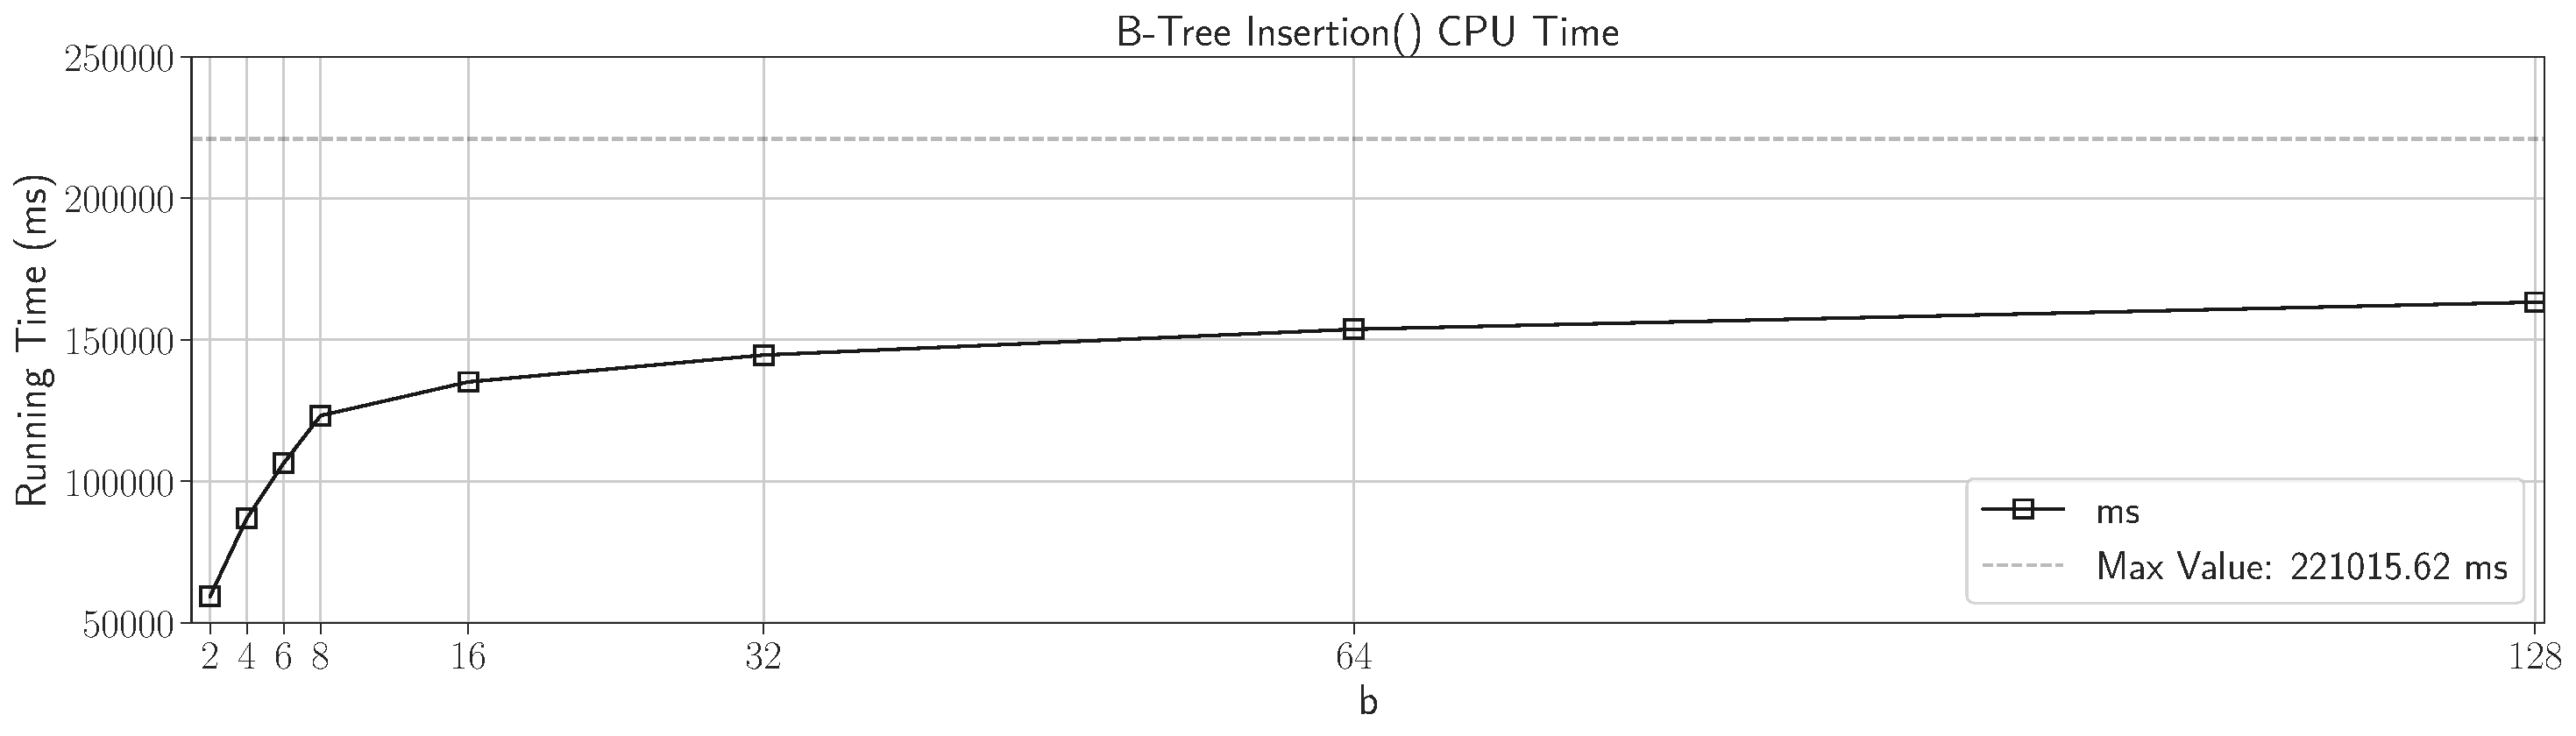
\includegraphics[width=\linewidth]{../notebook/b-tree_insertion()_cpu_time.pdf}
		\label{fig:cpu_time}
	\end{minipage}\hfill
	\\
	\begin{minipage}{1\textwidth}
		\centering
		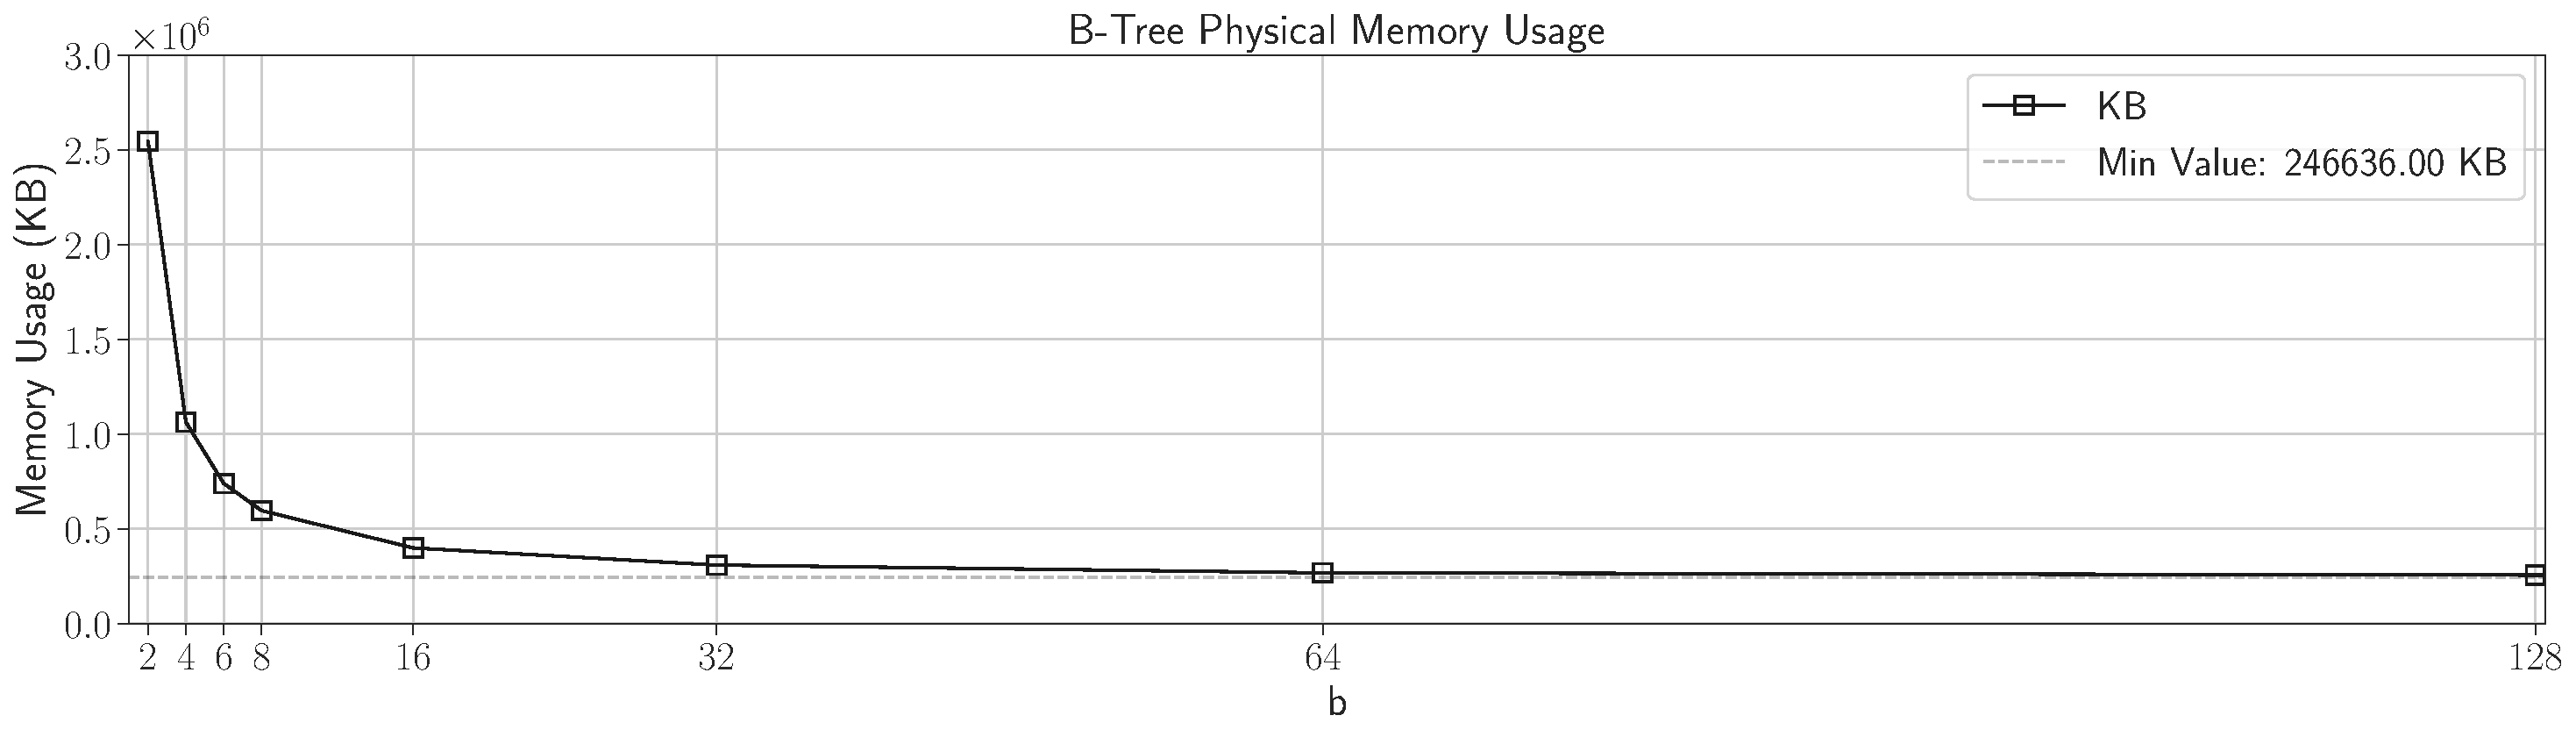
\includegraphics[width=\linewidth]{../notebook/b-tree_physical_memory_usage.pdf}
		\label{fig:physical_memory}
	\end{minipage}\hfill
	\caption{CPU Time and Physcal Memory Usage for B-Tree insertion with varying $b$ values.}
\end{figure}

Notice that as the parameter of $b$ the B-Tree increases, the physical memory usage decreases. This is strange, even when considering virtual memory (page file) usage. My theory is that increasing $b$ makes the tree shallower and more compact. Since a shallower tree reduces the number of pointers and improves spatial locality, nodes are more likely to fit within a cache line, leading to better memory efficiency?
\\\\
Anywhow... we want the b such that the it minimizes CPU time and memory used. They way I did it is to simply normalize CPU time and memory used and get closest b with to the smallest differnce. 

\begin{figure}[H]
	\centering
	\begin{minipage}{1\textwidth}
		\centering
		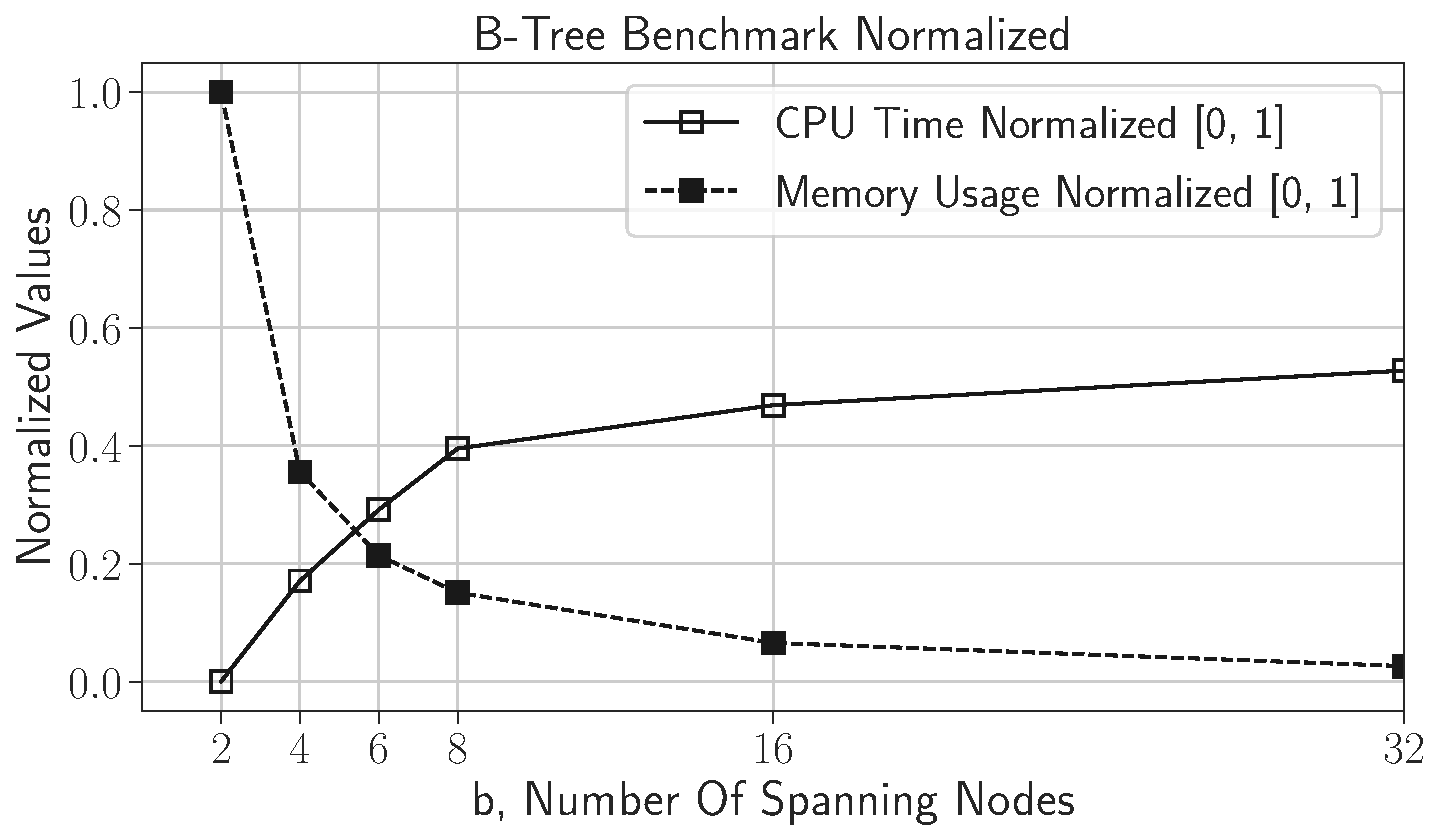
\includegraphics[width=\linewidth]{../notebook/b-tree_benchmark_normalized.pdf}
		\label{fig:benchmark_normalized}
	\end{minipage}
	\caption{Normalized CPU Time and Physcal Memory Usage comparison for B-Tree insertion with varying $b$ values.}
\end{figure}

Setting $b = 6$ gets the best overall performance. However, for applications that prioritize memory efficiency over execution time, a larger value, such as $b = 16$, could be more optimal, as the performance trade-off becomes less significant.

\subsubsection*{Comparing B-Tree and Builtin Ordered-Map Performance}



\vspace{2in} %Leave more space for comments!


\begin{thebibliography}{9}
	\bibitem{btree_github} 
	B-Tree Implementation on GitHub. 
	\textit{GitHub Repository}. 
	Available at: \url{https://github.com/frozenca/BTree}
\end{thebibliography}
	
\end{document}